\documentclass{report}
\usepackage{ptext}
\usepackage{lipsum}
\usepackage{graphicx}
\usepackage{ptext}

\input{Boostan-UserManual}

\newword{Abstraction}{Abstraction}
{انتزاع}{}

\newword{Abstract}{Abstract}
{انتزاعی}{}

\newword{AbsoluteMinimum}{Absolute Minimum}
{کمینه مطلق}{}


\newword{AcceptableCell}{Acceptable Cell}
{سلول پذیرفتنی}{سلول‌های پذیرفتنی}

\newword{AccessBurst}{Access Burst}
{توده دسترسی}{توده‌های دسترسی}


%%% S
\newword{Sample}{Sample}
{نمونه}{نمونه‌ها}

\newword{SamplePath}{Sample Path}
{نمونه مسیر}{}

\newword{SampleSpace}{Sample Space}
{فضای نمونه}{فضای نمونه‌ها}
\newacronym{ACK}{ACK}{Acknowledgement}

\newacronym{ACI}{ACI}{Application Control Interface}

\newacronym{ACIR}{ACIR}{Adjacent Channel Interference Ratio}

\newacronym{ACLC}{ACLC}{Adaptive Configuration of Logical Channels}

\newacronym{ACLP}{ACLP}{Adjacent Channel Leakage Power}

\title{مستند راه اندازی پروژه نهایی درس شبکه های تلفن همراه}
\type{مستند }
\author{زهرا دهقان\\اسماء حمید\\فاطمه شرح دهی مقدم}

\logofile{Pic/logo}


\begin{document}

\pagenumbering{gobble}
\Godpage
\maketitle
\pagenumbering{arabic}
\tableofcontents


\chapter{مقدمه}








\chapter{ \lr{Server-side Component}}
\section{راهنمای راه‌اندازی Polaris Server}

برای راه‌اندازی Polaris Server، ابتدا با دستور زیر یک Virtual Environment بسازید:

\begin{lstlisting}[language=bash]
python -m venv venv
\end{lstlisting}

سپس با استفاده از دستور زیر تمامی پکیج‌های مورد نیاز را نصب کنید:

\begin{lstlisting}[language=bash]
pip install -r requirements.txt
\end{lstlisting}

برای اجرای برنامه، از دستور زیر استفاده کنید:

\begin{lstlisting}[language=bash]
python manage.py runserver 0.0.0.0:8000
\end{lstlisting}

برای ایجاد یک ادمین، از دستور زیر استفاده کنید:

\begin{lstlisting}[language=bash]
python manage.py createsuperuser
\end{lstlisting}


\chapter{ \lr{Web Application}}

\chapter{ \lr{Android Mobile}}

\section{پیکربندی و راه‌اندازی اولیه اپلیکیشن}

برای اتصال اپلیکیشن به بک‌اند در محیط محلی، بک‌اند و موبایل باید در یک شبکه باشند. سپس آدرس IP سیستم میزبان بک‌اند را با دستور \textbf{ipconfig} در CMD پیدا کنید:

\vspace{0.3cm}

آدرس \lr{IPv4} را یادداشت کرده و در دو محل زیر جایگزین کنید:

\begin{enumerate}
	\item \textbf{SharedViewModel.kt}\\
	مسیر: \\
	\begin{latin}
		\texttt{app/src/main/java/com/example/Havanet/viewmodels/SharedViewModel.kt}\\
	\end{latin}
	مقدار موجود در خط شماره پانزده، عبارت از:
\begin{latin}
\begin{lstlisting}[mathescape=true, numbers=left, firstnumber=15]
val ip = "10.13.148.180"
\end{lstlisting}
\end{latin}
	را با IP جدید جایگزین کنید.
	
\item \textbf{network\_security\_config.xml}\\
	مسیر: \\
\begin{latin}
\texttt{app/src/main/res/xml/network\_security\_config.xml}\\
\end{latin}
	مقدار موجود در خط شماره چهار، عبارت از:
\begin{latin}
\begin{lstlisting}[mathescape=true, numbers=left, firstnumber=4]
<domain includeSubdomains="true">10.13.148.180</domain>
		\end{lstlisting}
	\end{latin}
	را با IP جدید جایگزین کنید.
\end{enumerate}

\vspace{0.5cm}

پس از انجام مراحل فوق، اپلیکیشن را با استفاده از \lr{Android Studio} روی دستگاه نصب کنید.

\section{مجوزهای موردنیاز}

اپلیکیشن برای عملکرد صحیح به مجوزهای مختلف نیاز دارد که در فایل \lr{AndroidManifest.xml} تعریف شده‌اند. برخی از این مجوزها هنگام اجرا از کاربر درخواست تأیید می‌شوند و باید آنها را قبول کند تا امکانات مربوط فعال شوند.

مجوزهای زیر هنگام اجرای برنامه از کاربر درخواست می‌شوند و باید حتماً اجازه داده شوند:

\begin{itemize}
	\item \lr{ACCESS\_FINE\_LOCATION}
	\item \lr{ACCESS\_COARSE\_LOCATION}
	\item \lr{READ\_PHONE\_STATE}
	\item \lr{SEND\_SMS}
	\item \lr{RECEIVE\_SMS}
\end{itemize}

سایر مجوزهای برنامه به صورت خودکار و بدون نیاز به تأیید کاربر فعال می‌شوند.

\section{صفحه ورود و ثبت‌نام}

پس از نصب و اجرای برنامه، صفحه \textbf{ورود/ثبت‌نام} نمایش داده می‌شود:

\begin{itemize}
	\item \textbf{ثبت‌نام:}\\
	کاربر باید ایمیل و رمز عبور خود را وارد کرده و اقدام به ایجاد حساب کاربری جدید نماید. رمز عبور باید حداقل شش کاراکتر داشته. درصورت داشتن اکانت، با لمس عبارت \textbf{«قبلاً ثبت‌نام کرده‌اید؟ وارد شوید.»} وارد صفحه ورود  شده.
	
	\item \textbf{ورود:}\\
	همانند صفحه ثبت نام با وارد کردن ایمیل و رمزعبور وارد امانت خود شده. درصورت نداشتن اکانت، با لمس عبارت \textbf{«حساب ندارید؟ ثبت‌نام کنید.»} وارد صفحه ورود  شده.
\end{itemize}

\section{محیط اصلی}

\subsection{تنظیمات}

برنامه تنظیمات به شما امکان می‌دهد رنگ‌ها و مقادیر سطح مربوط به آن‌ها را برای نمایش داده‌های شبکه تنظیم کنید. 
این تنظیمات در سه مرحله اصلی انجام می‌شود: انتخاب گزینه‌ها، انتخاب رنگ‌ها، و ثبت نهایی. 

\begin{itemize}
	\item \textbf{انتخاب گزینه‌ها} \\
	در بالای صفحه، سه بخش برای انتخاب گزینه‌های اصلی وجود دارد:
	
	\begin{itemize}
		\item \textbf{تکنولوژی}: یک منوی کشویی که به شما امکان انتخاب نوع شبکه را می‌دهد. گزینه‌های موجود عبارت‌اند از \lr{2G}،\lr{3G}،\lr{4G}،\lr{5G}.
		\item \textbf{ویژگی}: یک منوی کشویی برای انتخاب نوع داده. دو گزینه در این بخش وجود دارد: کیفیت و کمیت.
		\item \textbf{تعداد رنگ‌ها}: این منو به شما اجازه می‌دهد تعداد رنگ‌هایی که می‌خواهید برای نمایش داده‌ها استفاده کنید را از 3 تا 50 انتخاب کنید. با انتخاب هر عدد، محدوده مقادیر سطحی که می‌توانید برای رنگ‌ها تعیین کنید نیز به همان عدد محدود می‌شود.
	\end{itemize}
	
	\item \textbf{انتخاب رنگ‌ها و مقادیر سطح} \\
	بعد از انتخاب گزینه‌های اصلی، می‌توانید رنگ‌های مورد نظر خود را انتخاب کرده و برای هر رنگ یک مقدار سطح تعریف کنید:
	
	\begin{enumerate}
		\item \textbf{انتخاب رنگ}: از دایره رنگی بزرگ  که در وسط صفحه قرار دارد، رنگ مورد نظر خود را انتخاب کنید.
		\item \textbf{افزودن رنگ}: پس از انتخاب رنگ، دکمه «افزودن رنگ» را فشار دهید. یک پنجره جدید باز می‌شود که از شما می‌خواهد یک مقدار سطح برای آن رنگ وارد کنید. این مقدار باید یک عدد صحیح بین 1 تا تعداد رنگ‌هایی که در مرحله قبل انتخاب کرده‌اید، باشد. عدد وارد شده سطح
		\item \textbf{تأیید}: پس از وارد کردن مقدار سطح، دکمه «تأیید» را فشار دهید. حالا رنگ و سطح مربوط به آن در یک لیست در بالای دکمه «افزودن رنگ» نمایش داده می‌شود.
	\end{enumerate}
	
	\textbf{نکات مهم:}
	\begin{itemize}
		\item مقادیر سطح باید منحصر به فرد باشند. اگر مقدار سطحی را وارد کنید که قبلاً برای رنگ دیگری استفاده شده باشد، برنامه به شما اخطار می‌دهد.
		\item هرچه عدد سطح پایین‌تر باشد، به معنای وضعیت ضعیف‌تر (مثلاً کیفیت پایین‌تر یا سرعت کمتر) است؛ و هرچه عدد سطح بالاتر باشد، وضعیت بهتر را نشان می‌دهد.
		\item برای ویرایش رنگ‌ها کافی است روی مربعی که رنگ انتخابی شما را نشان می‌دهد کلیک کنید. یک حاشیه دور آن ظاهر می‌شود و می‌توانید از همان \lr{Color Picker} و دکمه «افزودن رنگ» برای تغییر رنگ یا مقدار سطح آن استفاده کنید. برای لغو ویرایش، مجدداً روی مربع کلیک کنید.
	\end{itemize}
	
	\item \textbf{ثبت نهایی} \\
	پس از اینکه تعداد رنگ‌های انتخابی شما به اندازه مقداری شد که در ابتدا انتخاب کرده‌اید (مثلاً اگر عدد 5 را انتخاب کرده‌اید و 5 رنگ اضافه کرده‌اید)، دکمه «ثبت نهایی» ظاهر می‌شود. با فشار دادن این دکمه، تمام تنظیمات شما (نوع تکنولوژی، ویژگی، تعداد رنگ‌ها، و لیست رنگ‌ها و سطوح) ذخیره و اعمال خواهد شد.
	
\end{itemize}

\begin{figure}[ht]
	\centering
	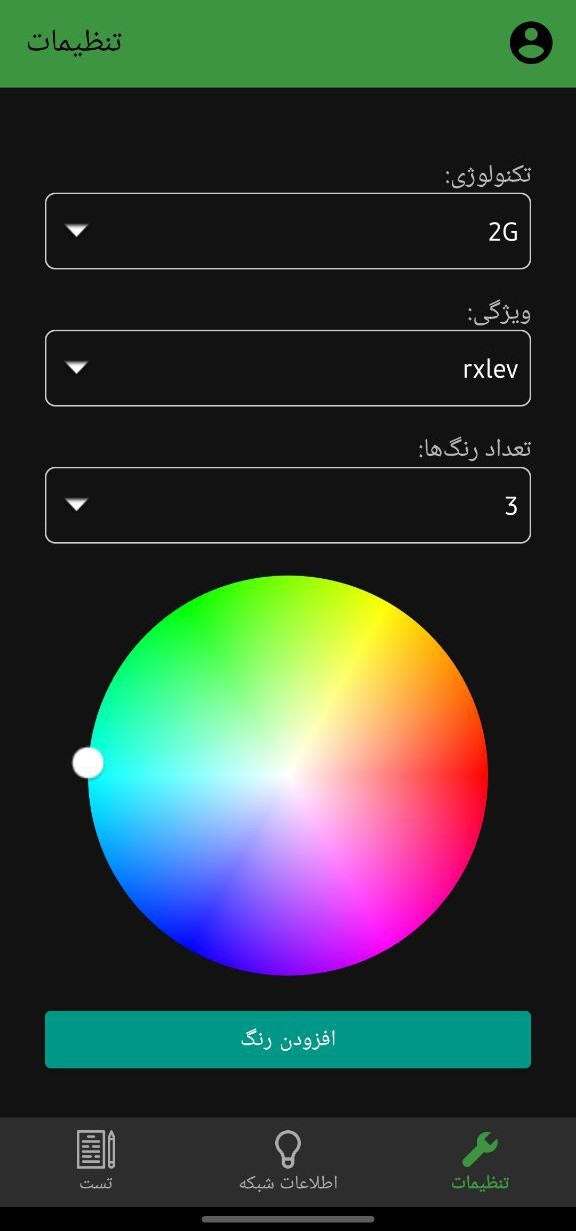
\includegraphics[width=0.7\textwidth,height=15cm,keepaspectratio]{Pic/setting}
	\caption{صفحه تنظیمات شبکه}
	\label{fig:setting}
\end{figure}

\subsection{اطلاعات شبکه}

در صفحه اطلاعات، وضعیت شبکه و موقعیت جغرافیایی کاربر به صورت زنده نمایش داده می‌شود.  
با فشردن دکمه \textbf{نمایش در نقشه}، موقعیت فعلی کاربر روی نقشه نشان داده می‌شود.

این اطلاعات به طور خودکار در پس‌زمینه به سرور ارسال می‌شوند و در همین صفحه می‌توان داده‌های ارسالی را مشاهده کرد.

\begin{figure}[ht]
	\centering
		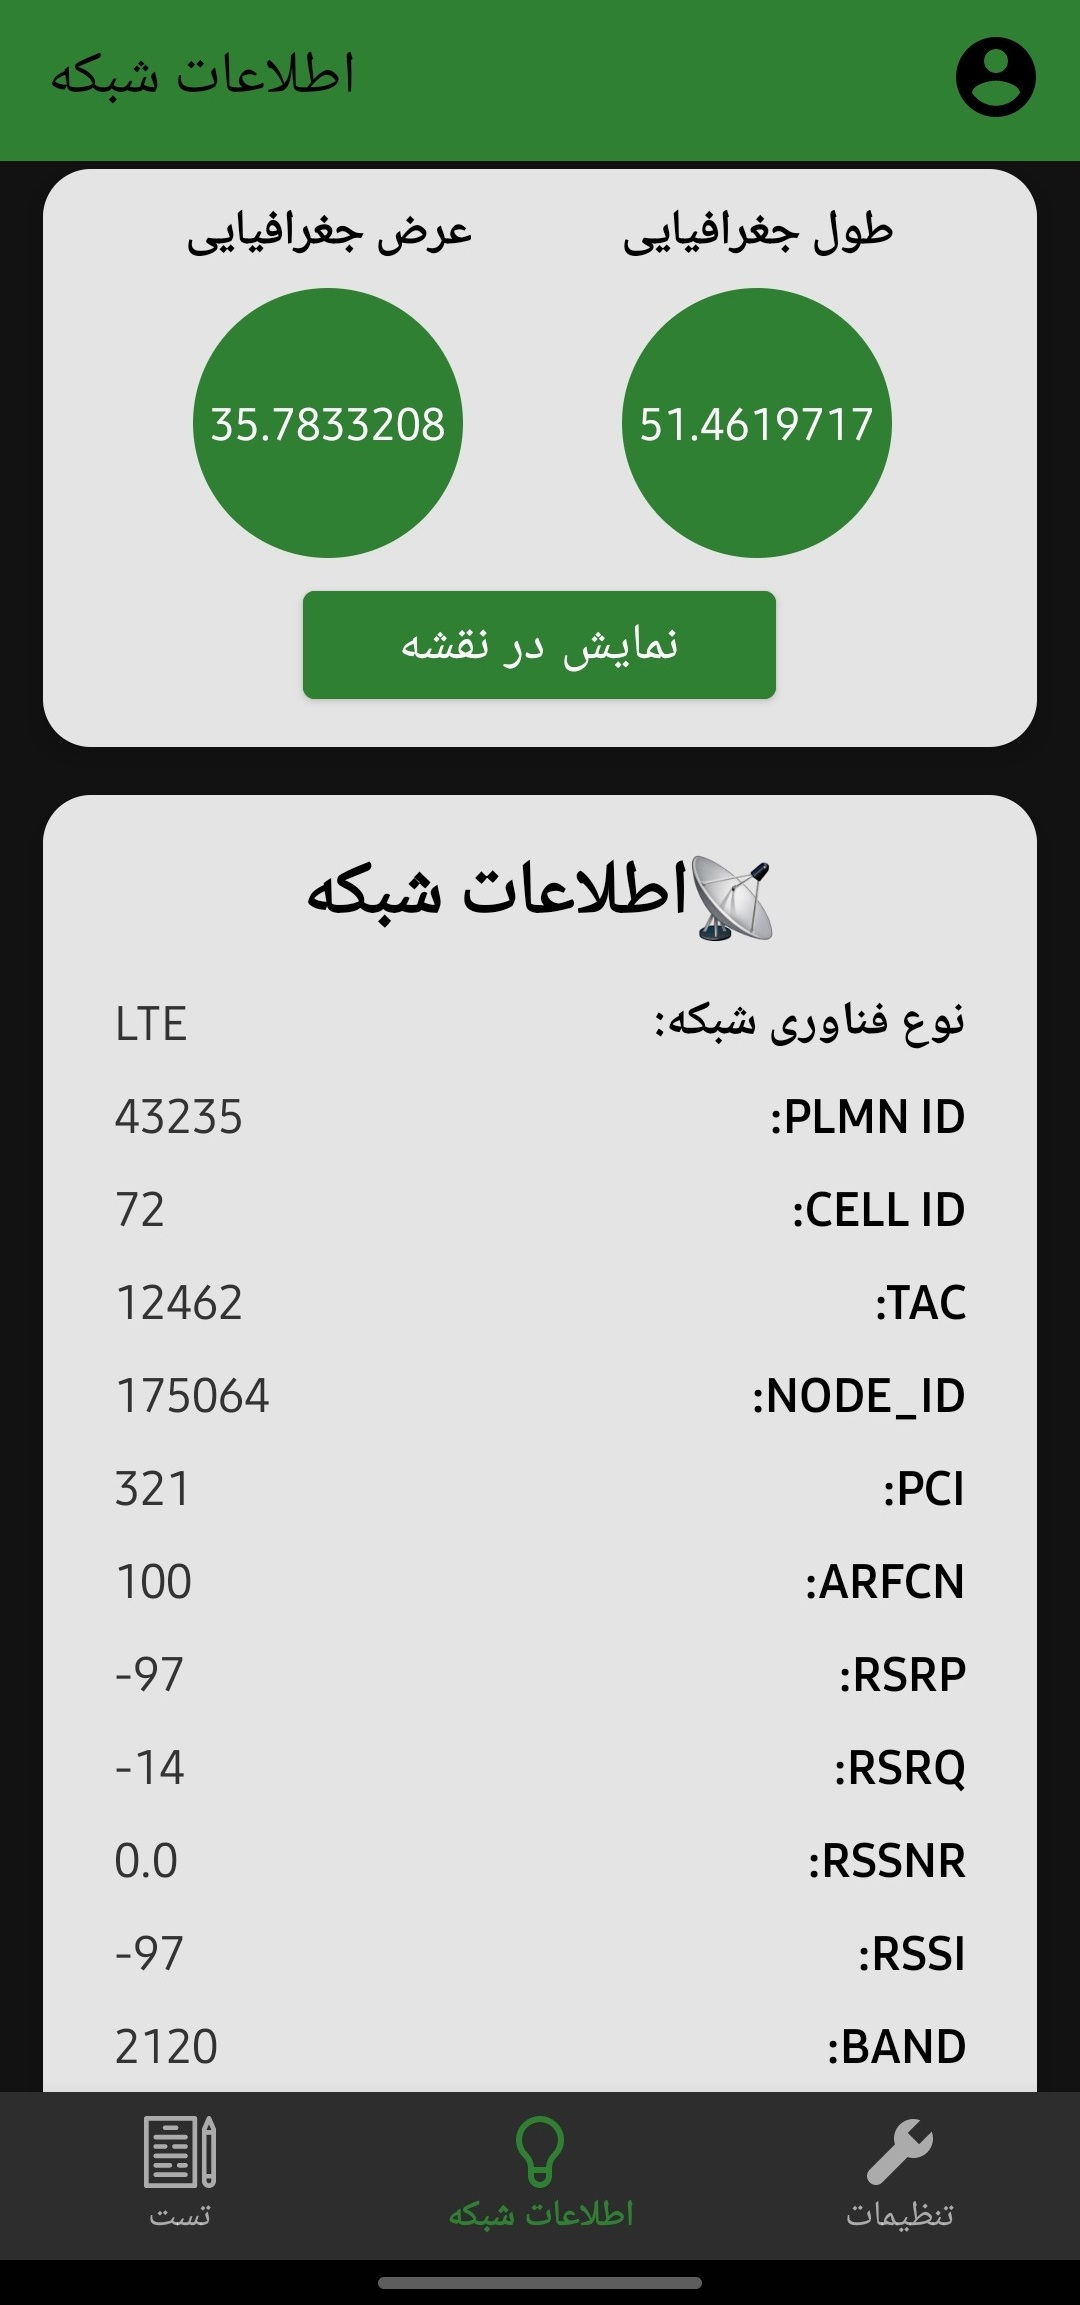
\includegraphics[width=0.7\textwidth,height=15cm,keepaspectratio]{Pic/info}
	\caption{صفحه اطلاعات شبکه}
	\label{fig:info}
\end{figure}

\subsection{تست‌ها}

با استفاده از این برنامه می‌توانید عملکرد و وضعیت شبکه اینترنت خود را با انجام تست‌های مختلف، به صورت دقیق بررسی کنید.

\begin{itemize}
	\item \textbf{بخش «تست‌های شبکه»} 

این بخش شامل شش دکمه برای انجام تست‌های مختلف شبکه است که می‌توانید به راحتی هر کدام را انتخاب و اجرا کنید.

\begin{itemize}
	\item \textbf{گذردهی دانلود (\lr{Download Throughput}):}\\
	با کلیک روی این دکمه، سرعت \textbf{دانلود داده} از سرور به گوشی شما سنجیده می‌شود. این تست برای ارزیابی عملکرد شبکه در هنگام دریافت فایل‌ها یا پخش ویدیو مفید است.
	
	\item \textbf{گذردهی آپلود (\lr{Upload Throughput}):}\\
	با کلیک روی این دکمه، سرعت \textbf{آپلود داده} از گوشی شما به سرور اندازه‌گیری می‌شود. این تست برای بررسی عملکرد شبکه در هنگام ارسال فایل‌ها یا آپلود تصاویر در شبکه‌های اجتماعی کاربرد دارد.
	
	\item \textbf{:Ping}\\
	این دکمه برای بررسی \textbf{زمان تأخیر (Latency)} در اتصال شبکه شما به یک سرور خاص به کار می‌رود. هرچه مقدار پینگ کمتر باشد، زمان پاسخ‌دهی شبکه بهتر است.
	
	\item \textbf{:DNS}\\
	این تست سرعت \textbf{پاسخ‌دهی سرور DNS} را می‌سنجد. DNS آدرس‌های وب ( \lr{www.google.com}) را به آدرس‌های IP ترجمه می‌کند. سرعت بالای پاسخ‌دهی DNS باعث لود شدن سریع‌تر صفحات وب می‌شود.
	
	\item \textbf{:Web}\\
	با کلیک روی این دکمه، عملکرد و سرعت \textbf{بارگذاری یک صفحه وب} مشخص تست می‌شود. این تست برای شبیه‌سازی تجربه واقعی کاربر هنگام مرور اینترنت طراحی شده است.
	
	\item \textbf{:SMS}\\
	این تست \textbf{سرعت ارسال پیامک (SMS)} را بررسی می‌کند. با این تست می‌توانید اطمینان حاصل کنید که سرویس پیامکی شما به درستی کار می‌کند.
\end{itemize}

\item \textbf{بخش «نتیجه تست»}  
در این بخش، نتایج تست‌های اجراشده نمایش داده می‌شود.\\
پیش از شروع هر تست، پیامی ظاهر می‌شود که از شما می‌خواهد روی دکمه موردنظر کلیک کنید.\\
هر تست در بازه‌ای دو دقیقه‌ای اجرا می‌شود و بین مراحل آن تأخیری ۱۰ ثانیه‌ای وجود دارد. 
به همین دلیل، پس از شروع یک تست، سایر دکمه‌ها تا پایان زمان دو دقیقه غیرفعال خواهند بود.\\

همچنین توجه داشته باشید که اگر هنگام اجرای تست از صفحه خارج شوید، فرآیند تست ناتمام باقی خواهد ماند.


\end{itemize}
 \begin{figure}[ht]
 	\centering
 	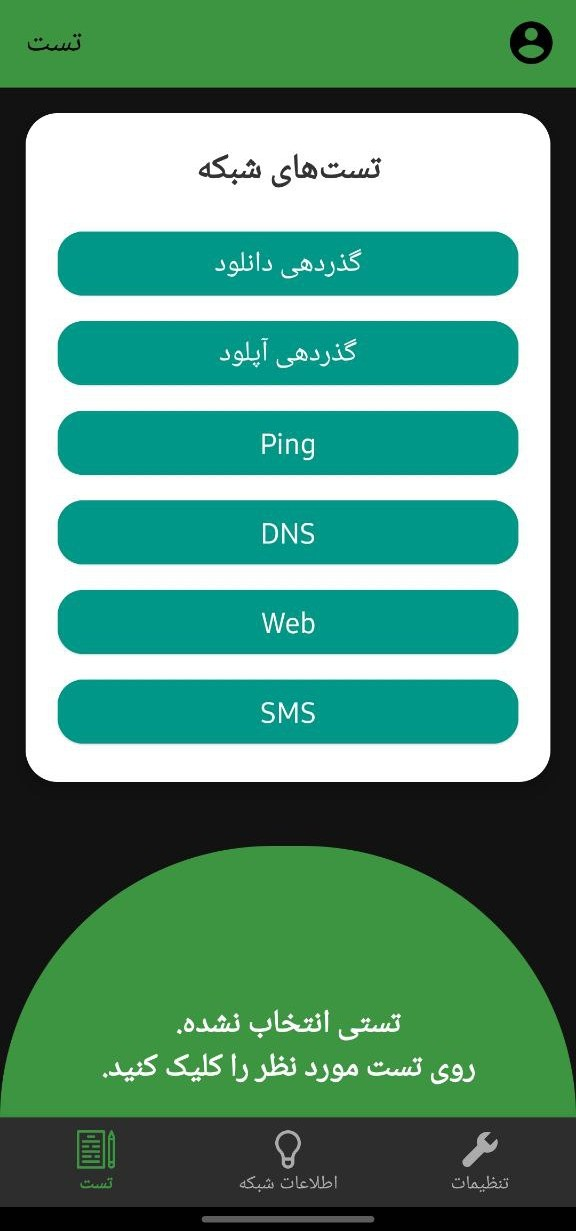
\includegraphics[width=0.7\textwidth,height=15cm,keepaspectratio]{Pic/test}
 	\caption{صفحه تست ها}
 	\label{fig:test}
 \end{figure}
\subsection{مدیریت حساب کاربری}

این صفحه به شما امکان می‌دهد اطلاعات حساب کاربری خود را مشاهده و مدیریت کنید.

\begin{itemize}
	\item \textbf{مشاهده و ویرایش اطلاعات حساب:}  
	در بخش میانی صفحه، سه فیلد برای نمایش اطلاعات شما وجود دارد:
	\begin{itemize}
		\item \textbf{نام کاربری:} نام کاربری فعلی شما را نشان می‌دهد.
		\item \textbf{ایمیل:} آدرس ایمیل شما که برای ورود به حساب استفاده می‌شود را نمایش می‌دهد.
		\item \textbf{رمز عبور:} رمز عبور شما به صورت محرمانه و با ستاره نمایش داده می‌شود.
	\end{itemize}
	برای ویرایش هر یک از این فیلدها، کافی است روی آیکون قلم که در سمت راست هر فیلد قرار دارد، ضربه بزنید.
	
	\item \textbf{خروج از حساب:}  
	در پایین صفحه، یک دکمه با عنوان \lr{Log Out} وجود دارد. با ضربه زدن روی این دکمه، شما از حساب کاربری خود خارج خواهید شد.
\end{itemize}

 
  \begin{figure}[ht]
 	\centering
 	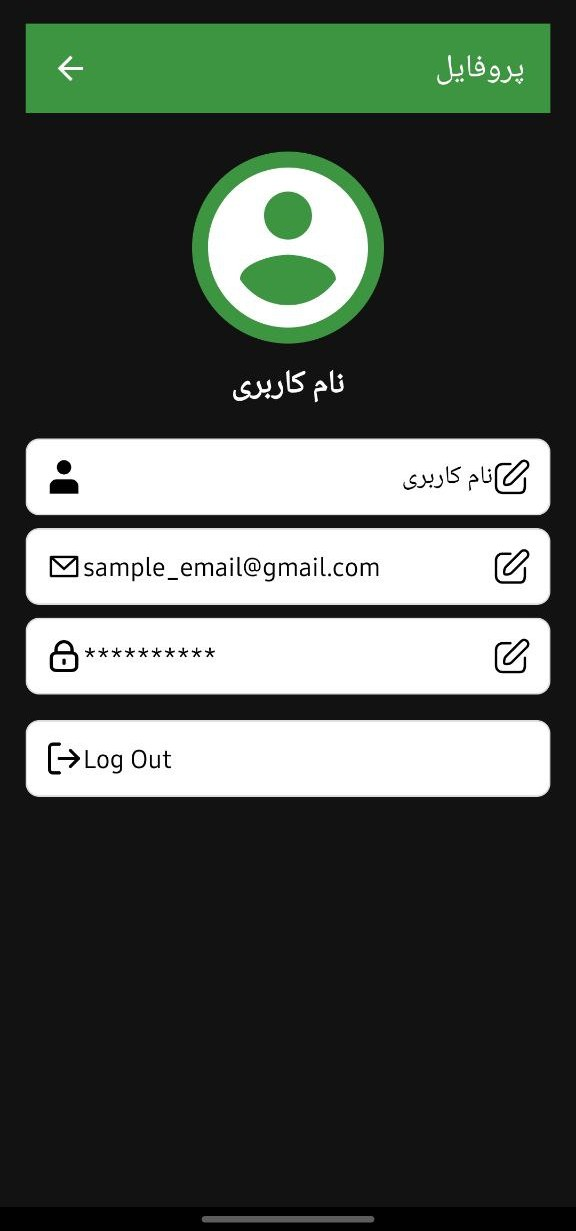
\includegraphics[width=0.7\textwidth,height=15cm,keepaspectratio]{Pic/profile}
 	\caption{صفحه حساب کاربری}
 	\label{fig:profile}
 \end{figure}
\end{document}



